

%#########################################

% author: S. Parisa Daj.
% email: s.dajkhosh@memphis.edu
% University of Memphis
% June 2020

%#########################################

\documentclass[12pt,oneside,geqno]{article}

\addtolength{\textheight}{120pt}
\oddsidemargin=-10pt
\topmargin=-.5in
\textwidth=6.5in
\pagestyle{empty}

% ######################## 	Packages
\usepackage{amssymb,latexsym,amsmath,amsthm}
\usepackage{amsfonts,raWFonts}
\usepackage{thmtools}
\usepackage{systeme}
\usepackage{mathtools}
\usepackage[usenames,dvipsnames]{color}
\usepackage{xcolor}
\usepackage{xfrac}
\usepackage{hyperref}
\usepackage[utf8]{inputenc}
\usepackage{enumerate}



\usepackage{listings}
\usepackage{xcolor}

\usepackage{graphicx}
\usepackage{caption}
\usepackage{subcaption}

% ######################## 	Colors
\definecolor{codegreen}{rgb}{0,0.6,0}
\definecolor{codegray}{rgb}{0.5,0.5,0.5}
\definecolor{codepurple}{rgb}{0.58,0,0.82}
\definecolor{backcolour}{rgb}{0.97,0.97,0.95}

% ######################## 	Style
\lstdefinestyle{mystyle}{
	backgroundcolor=\color{backcolour},   
	commentstyle=\color{codegreen},
	keywordstyle=\color{magenta},
	numberstyle=\tiny\color{codegray},
	stringstyle=\color{codepurple},
	basicstyle=\ttfamily\footnotesize,
	breakatwhitespace=false,         
	breaklines=true,                 
	captionpos=b,                    
	keepspaces=true,                 
	numbers=left,                    
	numbersep=5pt,                  
	showspaces=false,                
	showstringspaces=false,
	showtabs=false,                  
	tabsize=2
}

\lstset{style=mystyle}

\declaretheoremstyle[
headfont=\color{blue}\normalfont\bfseries,
notefont=\bfseries, 
notebraces={}{},
%bodyfont=\color{red}\normalfont\itshape,
bodyfont=\normalfont,%\itshape,
%headformat=\NUMBER.~\NAME\NOTE
headformat=\NAME\NOTE
]{colorejercicio}

\declaretheorem[
%numbered=no,
style=colorejercicio,
name=Problem
]{Problem}

% ######################## 	Document
\begin{document}
	
	\begin{center}
		{\LARGE EECE 8740-Neural Networks HW \#1}% Title
		\vspace*{1\baselineskip}   
		
		\scshape % Small caps
		\color{red}{(Solutions)}\\
		%  
		\vspace*{1\baselineskip}
		\color{black}University of Memphis\\[\baselineskip]
		%
		\vspace*{5\baselineskip} 
		
		Written by \\[\baselineskip]
		{\Large S. Parisa Daj.\par U00743495} \\
		(s.dajkhosh@memphis.edu)\\
		
		\vspace*{1\baselineskip}
		\today
	\end{center}
	%
	\clearpage
	
	
	%%%%%%%%%%%%%%%%%%%					1_question
	\begin{Problem}[a]
		Draw a computational graph for the following function and calculate values for
		a forward pass and backward passes: 
		
		\begin{align}
			\mathbf{y} = sigmoid(x1.w1 + max(x2, w2))
		\end{align}
	\end{Problem}
	
	%%%%%%%%%%%%%%%%%%%					1_solution
	\begin{proof}[\color{red}{Solution}]
		
		\begin{figure}
			\centering
			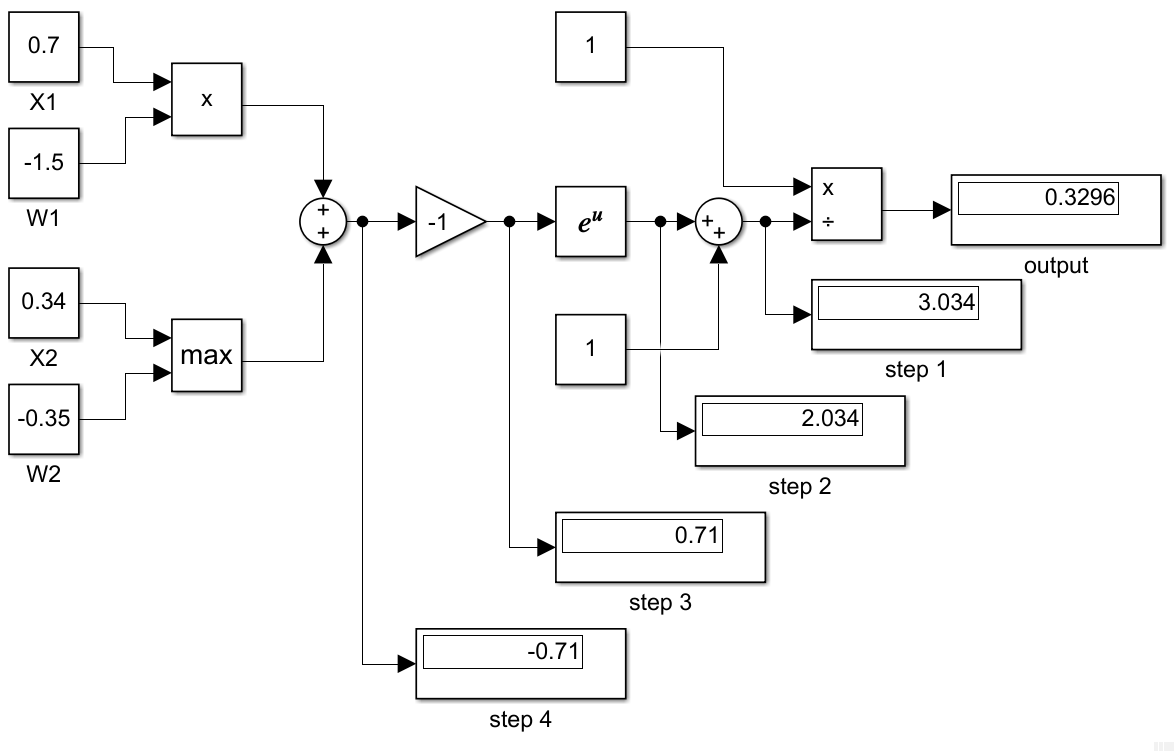
\includegraphics[width=\textwidth]{../figs/Q1_diagram.png}
			\caption{Schematic of the given equation in the question.}
			\label{img:net}
		\end{figure}
		
		The schematic of the given network is shown in (fig \ref{img:net}). Regarding to the given initial values for \(x_1\), \(w_1\), \(x_2\), and \(w_2\)  the forward pass calculations are done as follows:
		
		\begin{align}
			\mathbf{y} & = sigmoid(0.7 * (-1.5) + max(0.34, -0.35)) \\
			& = sigmoid(-10.5 + 0.34) \\
			& = sigmoid(-0.71)
		\end{align}
		
		Considering the fact that \(sigmoid(x)=\frac{1}{1 + e^{-x}}\)
		
		\begin{align}
			\mathbf{y} & = \frac{1}{1 + e^{0.71}} \\
			& = \frac{1}{1 + 2.034} \\
			& = \frac{1}{3.034} \\
			& = 0.3296
		\end{align}
		
		For the calculation of the backward pass, the local gradient can be calculated for each backward step. However, according to the lectures, instead of moving from step 1 to step 4 in (fig \ref{img:net}), there is a faster alternative solution. The derivative of the sigmoid function is known as \((1 - sigmoid(x)).sigmoid(x)\). Therefore, as follows the backward pass would be:
		
		\begin{align}
			\mathbf{step4} = (1) * ((1 - 0.3296) * (0.3296)) = 0.2210
		\end{align}
		
		Thus, the local gradients at each of the points after step 4 can be calculated as:
		
		\[\mathbf{step5} = (1) * (step4) = 0.2210 \] 
		\[\mathbf{x1_g} = (-1.5) * (step5) = 0.3314 \]  
		\[\mathbf{w1_g} = (0.7) * (step5) = 0.1547 \] 
		\[\mathbf{x2_g} = 0.34 \] 
		\[\mathbf{w2_g} = 0 \]
		
		
		These results were expected as multiplication at the beginning of the network stands for the gradient switcher. Also, the max function performs as the gradient router. Code Solutions for this question can also be found in \href{https://colab.research.google.com/drive/1O7_bI8X7BIBYwJ2gF5oAiFXH7jwp902a?authuser=1#scrollTo=ydX8Mu84z5oD}{this link}.
	\end{proof}
	
	
	%%%%%%%%%%%%%%%%%%%					2_question
	\begin{Problem}[b]
		
		\begin{itemize}
			
			\item Design and evaluate Deep Neural Network (DNN) models considering the following criteria:
			
			\begin{enumerate}[a)]
				
				\item Design two DNN models with following configuration:
				
				\begin{enumerate}[i)]
					
					\item 784 →150 →120 →10
					\item 784 →500 →250 → 100 →10
					
				\end{enumerate}
				
				\item Activation functions: sigmoid
				
				\item Use a SoftMax activation function for classification
				
				\item Categorical Cross-Entropy loss
				
				\item Number of epochs: 50 and
				
				\item Batch-size is 64.
				
			\end{enumerate}
			
			
			
			\item Evaluate the models with MNIST dataset:
			
			\begin{enumerate}[a)]
				\item Input image: 28x28 pixels (Gray scale images)
				
				\item Number of training samples: 60,000
				
				\item Number of testing samples: 10,000
				
				\item Number of classes: 10 (Handwritten digits).
				
			\end{enumerate}
			
			\item Write a report comparing two DNN models with training logs, testing errors, computational times, etc. 
		\end{itemize}
		
	\end{Problem}
	
	%%%%%%%%%%%%%%%%%%%					2_solution
	\begin{proof}[\color{red}{Solution}]
		
		\section{Introduction}
		Our goal in this assignment is to classify a group of handwritten digits with two deep learning neural networks. After that, we can compare the network architectures and determine which one is the best choice in this context. 
		
		First of all the data is loaded directly from the MNIST dataset. This dataset is loaded using Keras. The prepared data includes 60000 training samples and 10000 testing samples as expected by the question. Each data in the MNIST dataset is a \(28*28\) black and white picture indicating the handwriting of an English number between 0 and 9. Therefore, the output classes for this classification task will be 10.
		
		\section{Methodology and Deep Learning Architecture}
		
		Here there are two deep fully connected neural networks that are mostly similar. To clarify, both of them take pictures as input. Then, these inputs are passed to a sequential neural networks using Keras. To simplify the calculations, a flatten layer is taking the two-dimensional images into one-dimensional inputs for the network (size will be \(28*28=784\)). In the next step, the inputs have to pass through a number of fully connected hidden layers. As it is a classification task, the training loss function for all these layers is selected as the categorical cross-entropy loss. I believe that the reason that the sigmoid function is chosen as their activation function is for simplicity. Because, sigmoid limits the output, which can be helpful for the output layer, but not for the rest of the layers. The one possible explanation for me is that it might help us avoid exploding gradients. A SoftMax function is used in the output, to normalize the outputs between 0 and 1. this can help the classification process by finding the highest probability for each output to determine its class.
		
		The difference between the two networks is that the first network has two hidden layers; each with 150 and 120 neurons. However, the second network has more neurons with 3 hidden layers including 500, 250, and 100 neurons. Then, they both are trained in 50 epochs with a batch size of 64. 
		
		At the first sight, it seems that regarding our previous knowledge, the more complicated network with more hidden layers should have a better performance. But, we have to keep in mind that MNIST is known as a simple dataset. Therefore, a simplified network will be enough for detecting its classes, and a complex model might lead to over-fitting issues. To examine the initial understanding, there are two parameters that were not given from the question. I have selected them as follows: (Both Adam and SGD optimizers were tested, but as expected, Adam has better performance)
		
		\begin{align}
			\mathbf{learning rate} = 0.01 \\
			\mathbf{Optimizer} = Adam
		\end{align}
		
		\section{Experimental and Test Results}
		\begin{figure}
			\centering
			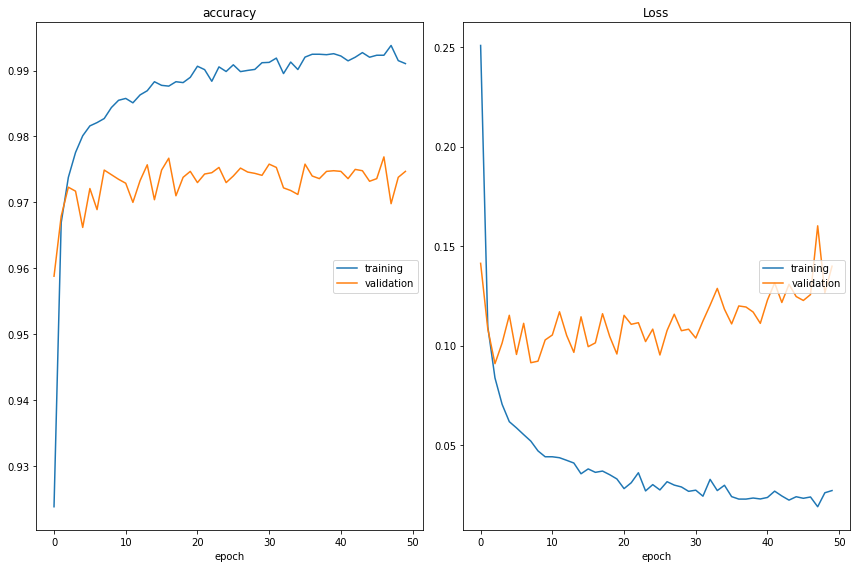
\includegraphics[width=\textwidth]{../figs/net_i.png}
			\caption{Accuracy and loss outputs per epoch for two hidden layers (training vs. test).}
			\label{img:net_i}
		\end{figure}
		
		(Fig \ref{img:net_i}) indicates that as mentioned in the above lines, with a simple two-layer network, very high accuracy is achieved. The fluctuations in the test accuracy determine that the learning rate has been chosen a bit big. A smaller learning rate can result in smoother output. However, it will decrease the increase rate of the accuracy, thus more epochs may be needed to reach the desired final accuracy. Moreover, in the 3 layer network shown in (fig \ref{img:net_ii}), we can see that the accuracy is high as well. The question which arises here is that is the final accuracy in the second network higher than the accuracy of the first network? Even if the answer is yes, does the difference worth the computational costs? 
		
		\begin{figure}
			\centering
			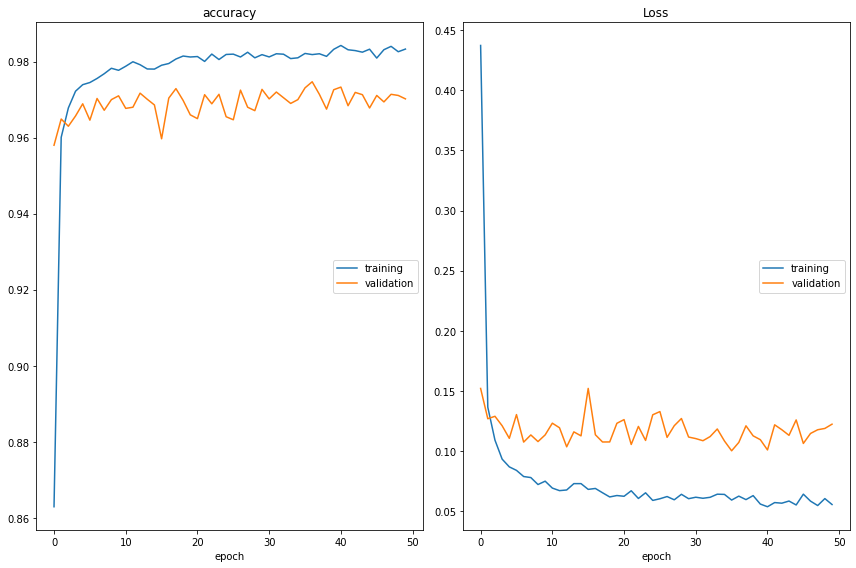
\includegraphics[width=\textwidth]{../figs/net_ii.png}
			\caption{Accuracy and loss outputs per epoch for three hidden layers (training vs. test).}
			\label{img:net_ii}
		\end{figure}
		
		To be able to answer the two asked questions, (fig \ref{img:loss}), (fig \ref{img:acc}), and (fig \ref{img:time}) in order show the comparison of test loss, test accuracy, and time between the two networks. As seen, not only we have lost a bit of accuracy in the more complex network, but we also spend a lot more time on achieving a similar, or even worse result. The one surprising result is that although the accuracy has been decreased in the second mode, the loss has also been decreased which is not explainable to me!
		
		\section{Conclusion}
		To conclude, this is the beginning of over-fitting in the network. Complexity is not always giving us more accurate outputs. In this case, the output is fitted to the labels too well, that it cannot avoid noisy data or handwriting mistakes in the MNIST dataset. This means that we have to take care of the complexity of our network. And I do not think it worths spending much more time and computational cost on a more complex network in this case. 
		
		The code is \href{https://colab.research.google.com/drive/1O7_bI8X7BIBYwJ2gF5oAiFXH7jwp902a?authuser=1#scrollTo=p_ujrM0L4yR9}{linked here}.
		\begin{figure}
			\centering
			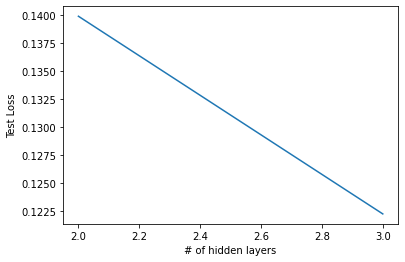
\includegraphics[width=10cm]{../figs/loss_comp.png}
			\caption{Comparing test loss for the layer with two hidden layers and the one with three hidden layers}
			\label{img:loss}
		\end{figure}
		
		
		\begin{figure}
			\centering
			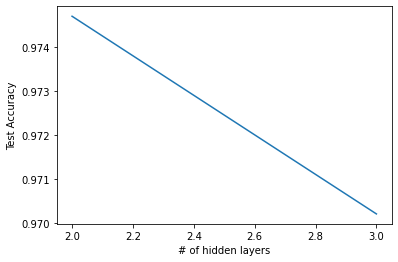
\includegraphics[width=10cm]{../figs/acc_comp.png}
			\caption{Comparing test accuracy for the layer with two hidden layers and the one with three hidden layers}
			\label{img:acc}
		\end{figure}
		
		
		\begin{figure}
			\centering
			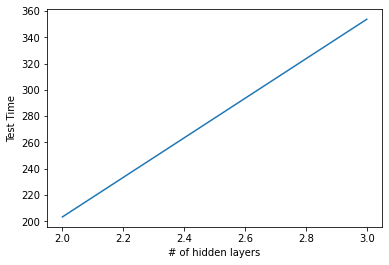
\includegraphics[width=10cm]{../figs/time_comp.png}
			\caption{Comparing time spent on the layer with two hidden layers and the one with three hidden layers}
			\label{img:time}
		\end{figure}

		
	\end{proof}
	%
	%\bibliography{bibfile} 
	%\bibliographystyle{ieeetr}
	
\end{document}